\documentclass[border=8pt,tikz]{standalone}
\usepackage{amsmath,amssymb}
\usepackage{tikz}
\usetikzlibrary{arrows.meta,calc,decorations.pathreplacing,patterns,shapes.geometric,positioning,shadings,decorations.markings,decorations.pathmorphing}

\begin{document}
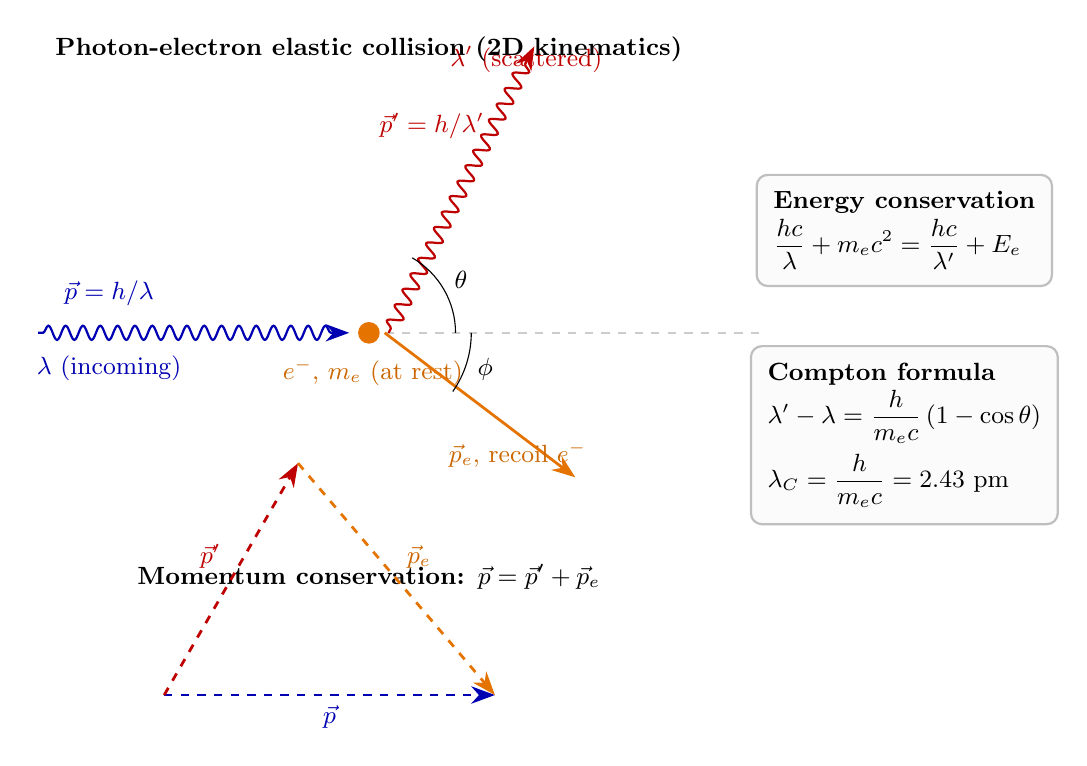
\begin{tikzpicture}[>={Stealth[length=3mm,width=2.2mm]},thick,
  photonIn/.style={blue!70!black,decorate,decoration={snake,amplitude=0.9mm,segment length=2.2mm,post length=1.8mm,pre length=0.6mm},->},
  photonOut/.style={red!75!black,decorate,decoration={snake,amplitude=0.9mm,segment length=2.2mm,post length=1.8mm,pre length=0.6mm},->},
  electron/.style={orange!90!black,->,line width=1pt},
  vec/.style={gray!70,dashed,->,line width=0.8pt},
  lbl/.style={font=\small}]

% ---------- Main collision diagram ----------
\begin{scope}

% incoming photon axis reference (dashed continuation)
\draw[gray!40,dashed,line width=0.5pt] (0,0) -- (5.0,0);

% Incoming photon (blue wavy) from left to collision point at (0,0)
\draw[photonIn] (-4.2,0) -- (-0.25,0);
\node[lbl,blue!70!black] at (-3.3,0.5) {$\vec p = h/\lambda$};
\node[lbl,blue!70!black] at (-3.3,-0.45) {$\lambda$ (incoming)};

% Collision point: electron (orange filled circle)
\filldraw[orange!90!black] (0,0) circle (3.5pt);
\node[lbl,orange!80!black] at (0.05,-0.5) {$e^-$, $m_e$ (at rest)};

% Scattered photon: angle theta ~ 60 deg above horizontal
\def\thetaAng{60}
\draw[photonOut] (0.25,0) -- ({4.2*cos(\thetaAng)},{4.2*sin(\thetaAng)});
\node[lbl,red!75!black] at ({2.4*cos(\thetaAng)-0.4},{2.4*sin(\thetaAng)+0.55}) {$\vec p' = h/\lambda'$};
\node[lbl,red!75!black] at ({3.6*cos(\thetaAng)+0.2},{3.6*sin(\thetaAng)+0.35}) {$\lambda'$ (scattered)};

% Recoil electron: angle phi below horizontal on other side
\def\phiAng{-35}
\draw[electron] (0.2,0) -- ({3.2*cos(\phiAng)},{3.2*sin(\phiAng)});
\node[lbl,orange!80!black] at ({2.0*cos(\phiAng)+0.25},{2.0*sin(\phiAng)-0.4}) {$\vec p_e$, recoil $e^-$};

% Angle arc for theta (between +x axis and scattered photon)
\draw[black,thin] (1.1,0) arc (0:\thetaAng:1.1);
\node[lbl] at ({1.35*cos(\thetaAng/2)},{1.35*sin(\thetaAng/2)}) {$\theta$};

% Angle arc for phi (between +x axis and recoil electron direction, below)
\draw[black,thin] (1.3,0) arc (0:\phiAng:1.3);
\node[lbl] at ({1.55*cos(\phiAng/2)},{1.55*sin(\phiAng/2)}) {$\phi$};

% Title of upper scene
\node[lbl,font=\small\bfseries] at (0,3.6) {Photon-electron elastic collision (2D kinematics)};

\end{scope}

% ---------- Momentum triangle (below) ----------
\begin{scope}[yshift=-4.6cm,xshift=0cm]

\node[lbl,font=\small\bfseries] at (0,1.5) {Momentum conservation: $\vec p = \vec p' + \vec p_e$};

% Place the triangle
% p (incoming) horizontal
\coordinate (A) at (-2.6,0);
\coordinate (B) at (1.6,0);
% p' at angle theta from A's tip? Actually: p = p' + p_e means tip-to-tail: from A go p' then p_e to reach B.
% Put p' from A to C, then p_e from C to B.
\def\pLen{4.2} % |p|
\def\pPrimeLen{3.4} % |p'| slightly smaller (red-shifted)
\def\thetaTri{60}
\coordinate (C) at ($(A)+({\pPrimeLen*cos(\thetaTri)},{\pPrimeLen*sin(\thetaTri)})$);

% Draw p (incoming, blue) A->B
\draw[vec,blue!70!black,line width=1pt] (A) -- (B) node[midway,below,lbl,blue!70!black]{$\vec p$};

% Draw p' (red) A->C
\draw[vec,red!75!black,line width=1pt] (A) -- (C) node[midway,above left,lbl,red!75!black]{$\vec p'$};

% Draw p_e (orange) C->B
\draw[vec,orange!90!black,line width=1pt] (C) -- (B) node[midway,above right,lbl,orange!80!black]{$\vec p_e$};

\end{scope}

% ---------- Formula box on the right ----------
\begin{scope}[xshift=6.8cm,yshift=0cm]

\node[draw=gray!50,rounded corners,inner sep=6pt,align=left,fill=gray!3,lbl] at (0,1.3) {%
\textbf{Energy conservation}\\[1pt]
$\dfrac{hc}{\lambda} + m_e c^2 = \dfrac{hc}{\lambda'} + E_e$};

\node[draw=gray!50,rounded corners,inner sep=6pt,align=left,fill=gray!3,lbl] at (0,-1.3) {%
\textbf{Compton formula}\\[1pt]
$\lambda' - \lambda = \dfrac{h}{m_e c}\,(1-\cos\theta)$\\[3pt]
$\lambda_C = \dfrac{h}{m_e c} = 2.43\ \mathrm{pm}$};

\end{scope}

\end{tikzpicture}
\end{document}
